\documentclass[10pt]{article}
\usepackage{icmlko}

\icmlmeta{IP 파운데이션 월드모델}{302}{섞어도 똑같이 듣는다}{하네스에서 유일하게 복제된 층에 위약을 붙였다 --- 신호를 앵커 사이에서 뒤섞어도 이득이 그대로다}

\begin{document}

\twocolumn[
\icmlheader

\begin{abstract}
노트 298에서 하네스의 세 층 중 \textbf{신호 하나만} 복제됐다(새 21건에서
$+$0.2160, $t{=}2.21$). 그런데 그 신호 삼종 중 \textbf{어느 것도 앵커 자신의
일평균을 못 가른다} --- 완판 $\rho{=}0.085$($p{=}0.23$) · 대기 $-$0.014 ·
예약 0.013, 카테고리 안에서 중심화한 뒤에도 마찬가지다. 정보가 앵커 성과를
못 가르는데 빼면 예측이 나빠진다면 이득이 신호의 \emph{내용}이 아니라
\emph{모양}일 수 있다(노트 133). \textbf{위약 팔}을 만들었다 --- 신호 삼종을
앵커들 사이에서 \textbf{치환}한다. 주변 분포와 프롬프트 모양이 정확히 같고
앵커와의 짝만 깨진다(짝이 그대로인 것 34/229). 시점으로 자른 \emph{뒤에}
섞는다. 척도 · 문턱 · 실패 조건을 재기 전에 못 박고
(\texttt{preregister\_placebo.json}) 48건에 돌렸다. 결과 --- \textbf{진짜 대
위약 $t{=}{-}0.59$(미달)} · \textbf{위약 대 제거 $t{=}{+}2.52$(통과)}.
\textbf{내용을 통째로 부수어도 이득이 안 준다.} APE 중앙값도 진짜 0.400 ·
위약 0.444 · 제거 0.520 으로 앞의 둘이 붙어 있다. 미리 적은 두 가설 중
\textbf{`모양'이 맞았다.} 하네스에서 유일하게 살아남은 이득이 \textbf{어느
앵커가 완판했는지와 무관}하다 --- 뱅크에 수요신호 칸이 \emph{있다}는 것이
일하지, 그 칸이 \emph{누구 것인지}는 안 읽힌다.
\end{abstract}
]

\section{복제된 층이 아무것도 안 가른다}

노트 298이 하네스 짝 셋을 사전 등록해 복제했고 \textbf{신호 하나만} 살았다.
그 층이 무엇인지 봤다 --- \texttt{market\_bank.\_line} 이 앵커 줄에 붙이는
\textbf{완판 · 대기 · 예약} 셋이다.

\begin{center}\footnotesize
\begin{tabular}{lrrr}
\hline
앵커 201건 & 덮음 & $\rho$(일평균) & $p$ \\
\hline
완판 & 32\% & 0.085 & 0.23 \\
대기 & 39\% & $-$0.014 & 0.84 \\
예약 & 27\% & 0.013 & 0.85 \\
\hline
\multicolumn{4}{l}{카테고리 안에서 중심화한 뒤} \\
완판 & & 0.065 & 0.36 \\
대기 & & $-$0.031 & 0.67 \\
예약 & & $-$0.031 & 0.66 \\
\hline
\end{tabular}
\end{center}

\textbf{아무것도 안 가른다.} 대조로, 같은 뱅크에서 카테고리는
$H{=}28.8$($p{=}0.0002$)로 다섯 배를 가른다(노트 299).

\paragraph{두 가설을 적었다} \textbf{내용} --- 신호가 무언가를 말하고 모형이
그것을 읽는다. \textbf{모양} --- 이득은 그 칸이 \emph{있다}는 데서 오고
내용은 안 읽힌다. \textbf{예상은 모양 쪽으로 적었다.}

\paragraph{그리고 결과 보기 전에 세 번째 경로도 죽였다} 신호가 \emph{라벨
신뢰도}의 대리일 가능성 --- 신호 유무가 등급과 붙긴 하는데($p{=}0.024$)
\textbf{거꾸로}다(등급 B 56\% · C 76\% · E 71\%). 잘 잰 앵커를 가리키는 게
아니다.

\section{위약 팔}

\begin{figure*}[t]
\centering
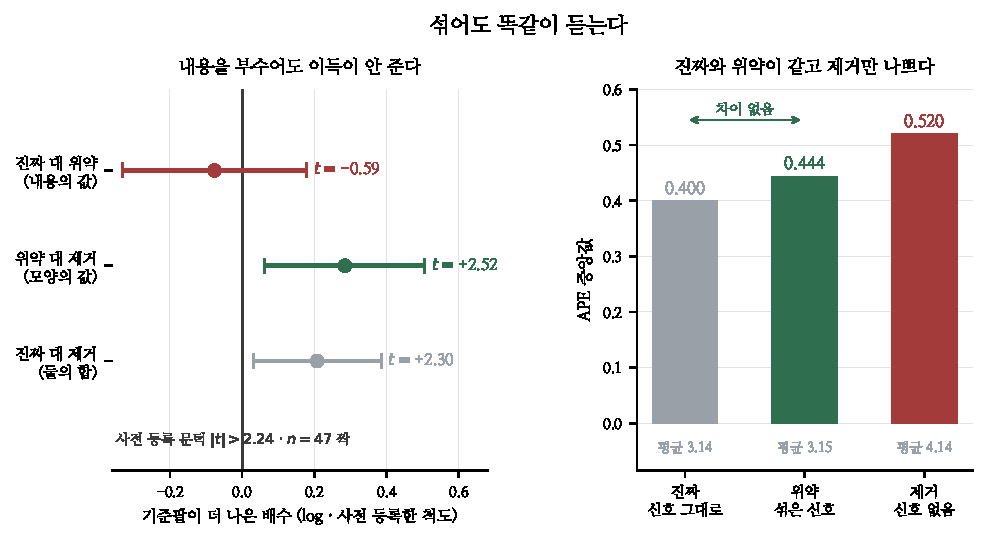
\includegraphics[width=\textwidth]{figs/placebo.pdf}
\caption{왼쪽 --- 사전 등록한 척도로 잰 세 짝 비교($\pm$1.96\,짝SE).
오른쪽 --- 세 팔의 APE.}
\end{figure*}

신호 삼종을 앵커들 사이에서 \textbf{치환}한다(\texttt{market\_bank.
shuffle\_signals}, 씨앗 1234).

\begin{center}\footnotesize
\begin{tabular}{lr}
\hline
확인 & \\
\hline
주변 분포 같음 & \textbf{True} \\
짝이 그대로인 것 & 34 / 229 (15\%) \\
두 번 불러 같은가 & \textbf{True} \\
\hline
\end{tabular}
\end{center}

\textbf{자른 뒤에 섞는다.} 전체에서 섞고 시점으로 자르면 팔마다 남는 신호의
분포가 달라져 \emph{모양이 안 맞고}, 그러면 위약이 아니다.

\section{내용을 부수어도 이득이 안 준다}

사전 등록한 척도($\log\frac{\text{비교팔 APE}+0.05}{\text{기준팔 APE}+0.05}$)와
문턱($|t|{>}z(0.05/4){=}2.24$)으로 읽었다. 48건 중 47건이 세 팔을 다 가졌다.

\begin{center}\small
\begin{tabular}{lrrrl}
\hline
비교 & 효과 & 짝SE & $t$ & \\
\hline
\textbf{진짜 대 위약} & $-$0.0763 & 0.1302 & \textbf{$-$0.59} & 미달 \\
\textbf{위약 대 제거} & $+$0.2843 & 0.1129 & \textbf{$+$2.52} & \textbf{통과} \\
진짜 대 제거 & $+$0.2080 & 0.0902 & $+$2.30 & 통과 \\
\hline
\end{tabular}
\end{center}

\begin{center}\footnotesize
\begin{tabular}{lrr}
\hline
팔 & APE 중앙 & APE 평균 \\
\hline
진짜 (신호 그대로) & 0.400 & 3.142 \\
\textbf{위약 (섞은 신호)} & \textbf{0.444} & \textbf{3.150} \\
제거 (신호 없음) & 0.520 & 4.145 \\
\hline
\end{tabular}
\end{center}

\textbf{진짜와 위약이 붙어 있고 제거만 떨어진다.} 미리 적은 두 가설 중
\textbf{`모양'이 맞았다.}

\paragraph{무엇이 부서졌고 무엇이 남았나} 치환은 \textbf{어느 앵커가
완판했는지}를 완전히 지운다(짝이 남은 것 15\%). 남는 것은 \textbf{뱅크의
66\%에 수요신호 칸이 있다}는 사실과 그 칸들의 총량 · 배치다. \textbf{그것만
있으면 이득이 다 나온다.}

\section{그래서 무엇을 배웠나}

\paragraph{① 이 이득은 자료의 값어치가 아니다} 노트 298이 ``남은 것은
신호 층 하나''로 끝나면서 다음 수를 ``어느 신호가 듣나 --- 아직 뭉치다''로
적었다. \textbf{그 물음이 잘못 놓였다.} 셋 중 어느 것도 아니고, 셋을
아무렇게나 섞어도 같다. \textbf{신호를 더 잘 모으는 것은 이 이득을 안
키운다.}

\paragraph{② 절제 실험이 자료를 재고 있지 않았다} 하네스의 세 팔
(\texttt{nomkt} · \texttt{nofeat} · \texttt{nosig})은 전부 \textbf{프롬프트에서
무언가를 지우는} 방식이다. 지우면 내용과 모양이 같이 사라진다. \textbf{위약
없이는 둘을 못 가른다.} 노트 295$\sim$298이 잰 것 전부가 이 혼동을 안고
있었을 수 있다 --- 시장층과 피처에도 같은 위약을 붙여야 안다.

\paragraph{③ 그런데 이득 자체는 진짜다} 위약 대 제거가 $t{=}2.52$ 로 문턱을
넘는다. \textbf{그 칸이 있으면 예측이 나아진다} --- APE 중앙 0.520 $\to$
0.444. 왜인지는 이 노트가 답 못 한다. 후보: 줄이 길어져 앵커가 더 오래
붙들린다 · 형식이 촘촘해져 표를 표로 읽는다 · 신호 칸의 유무가 그 앵커의
\emph{기록 밀도}를 알린다.

\paragraph{남은 것}
\begin{center}\small
\begin{tabular}{ll}
\hline
갈래 & 왜 \\
\hline
시장층 · 피처에 위약 & 같은 혼동을 안고 있다 \\
빈 칸을 채워 보기 & ``\texttt{-}'' 로 자리만 두면? \\
길이만 늘려 보기 & 모양의 어느 부분인가 \\
도메인별 빌림 & 노트 301의 갈래 --- 돌고 있다 \\
\hline
\end{tabular}
\end{center}

\paragraph{규약} \textbf{지워서 잰 것은 위약으로 다시 재라.} 절제는 편하고
싸지만 \textbf{내용과 모양을 같이 지운다.} 치환은 모양을 그대로 두고 내용만
지우므로 둘을 가른다 --- 그리고 이 판에서는 \textbf{모양이 전부였다.}
그리고 \textbf{이득이 복제된다고 해서 그 이득의 원인을 안다는 뜻이 아니다}
--- 노트 298이 신호 층을 두 번 독립으로 확인했는데, 두 번 다 확인한 것은
``신호 칸을 지우면 나빠진다''이지 ``신호가 정보를 나른다''가 아니었다.

\end{document}
